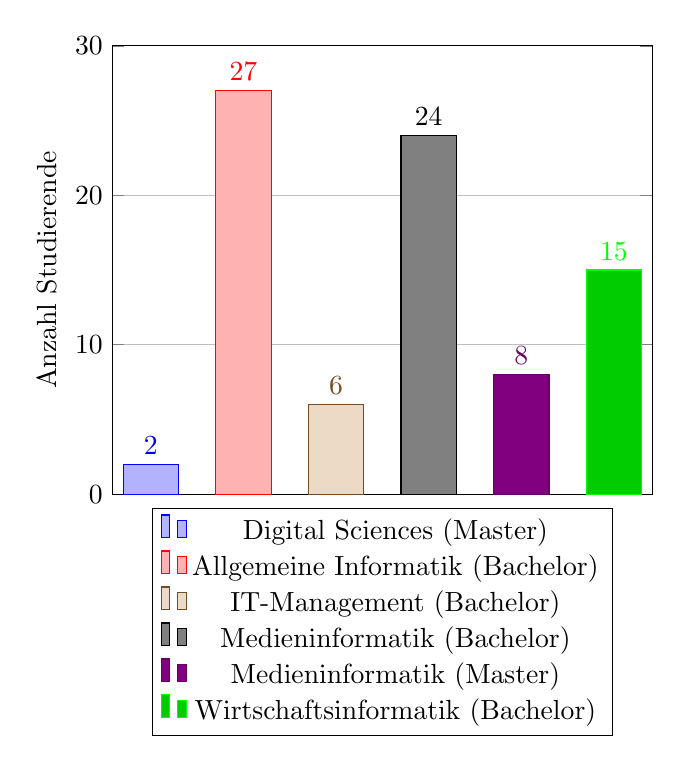
\begin{tikzpicture}
    \begin{axis}[
            x tick label style={
                /pgf/number format/1000 sep=},
            ylabel=Anzahl Studierende,
            enlarge x limits=1.2,
            ymax=30,
            ymin=0,
            legend style={at={(0.5,-0.03)},
            anchor=north,legend columns=1},
            ybar,
            bar width=20pt,
            xticklabels={},
            xtick=\empty,
            nodes near coords,
            grid=major,
        ]
        
        \addplot coordinates {(1,2)}; % DS
        \addplot coordinates {(2,27)}; % AI
        \addplot coordinates {(3,6)}; % ITM
        \addplot coordinates {(4,24)}; % MIB
        \addplot coordinates {(5,8)}; % MIM
        \addplot coordinates {(6,15)}; % WI
        
        \legend{Digital Sciences (Master), Allgemeine Informatik (Bachelor), IT-Management (Bachelor), Medieninformatik (Bachelor), Medieninformatik (Master), Wirtschaftsinformatik (Bachelor)}
    \end{axis}
\end{tikzpicture}